\documentclass[hidelinks,12pt]{article}
\usepackage[left=0.25cm,top=1cm,right=0.25cm,bottom=1cm]{geometry}
%\usepackage[landscape]{geometry}
\textwidth = 20cm
\hoffset = -1cm
\usepackage[utf8]{inputenc}
\usepackage[spanish,es-tabla]{babel}
\usepackage[autostyle,spanish=mexican]{csquotes}
\usepackage[tbtags]{amsmath}
\usepackage{nccmath}
\usepackage{amsthm}
\usepackage{amssymb}
\usepackage{mathrsfs}
\usepackage{graphicx}
\usepackage{subfig}
\usepackage{standalone}
\usepackage[outdir=./Imagenes/]{epstopdf}
\usepackage{siunitx}
\usepackage{physics}
\usepackage{color}
\usepackage{float}
\usepackage{hyperref}
\usepackage{multicol}
%\usepackage{milista}
\usepackage{anyfontsize}
\usepackage{anysize}
%\usepackage{enumerate}
\usepackage[shortlabels]{enumitem}
\usepackage{capt-of}
\usepackage{bm}
\usepackage{relsize}
\usepackage{placeins}
\usepackage{empheq}
\usepackage{cancel}
\usepackage{wrapfig}
\usepackage[flushleft]{threeparttable}
\usepackage{makecell}
\usepackage{fancyhdr}
\usepackage{tikz}
\usepackage{bigints}
\usepackage{scalerel}
\usepackage{pgfplots}
\usepackage{pdflscape}
\pgfplotsset{compat=1.16}
\spanishdecimal{.}
\renewcommand{\baselinestretch}{1.5} 
\renewcommand\labelenumii{\theenumi.{\arabic{enumii}})}
\newcommand{\ptilde}[1]{\ensuremath{{#1}^{\prime}}}
\newcommand{\stilde}[1]{\ensuremath{{#1}^{\prime \prime}}}
\newcommand{\ttilde}[1]{\ensuremath{{#1}^{\prime \prime \prime}}}
\newcommand{\ntilde}[2]{\ensuremath{{#1}^{(#2)}}}

\newtheorem{defi}{{\it Definición}}[section]
\newtheorem{teo}{{\it Teorema}}[section]
\newtheorem{ejemplo}{{\it Ejemplo}}[section]
\newtheorem{propiedad}{{\it Propiedad}}[section]
\newtheorem{lema}{{\it Lema}}[section]
\newtheorem{cor}{Corolario}
\newtheorem{ejer}{Ejercicio}[section]

\newlist{milista}{enumerate}{2}
\setlist[milista,1]{label=\arabic*)}
\setlist[milista,2]{label=\arabic{milistai}.\arabic*)}
\newlength{\depthofsumsign}
\setlength{\depthofsumsign}{\depthof{$\sum$}}
\newcommand{\nsum}[1][1.4]{% only for \displaystyle
    \mathop{%
        \raisebox
            {-#1\depthofsumsign+1\depthofsumsign}
            {\scalebox
                {#1}
                {$\displaystyle\sum$}%
            }
    }
}
\def\scaleint#1{\vcenter{\hbox{\scaleto[3ex]{\displaystyle\int}{#1}}}}
\def\bs{\mkern-12mu}



\title{Teorema de adición de los armónicos esféricos \\ {\large Tema 4}\vspace{-3ex}}
\author{M. en C. Gustavo Contreras Mayén}
\date{ }

\pagestyle{fancy}
\fancyhf{}
\rhead{Curso MAF}
\lhead{\leftmark}
\rfoot{\thepage}
\setlength{\headheight}{16pt}%

\def\changemargin#1#2{\list{}{\rightmargin#2\leftmargin#1}\item[]}
\let\endchangemargin=\endlist 


\begin{document}
\maketitle
\fontsize{14}{14}\selectfont
\tableofcontents
\newpage

\section{La fórmula de adición.}

Supongamos que tenemos dos vectores:
\begin{align}
\va{r} = (r, \theta, \phi) \hspace{1.5cm} \va{r}^{\, \prime} (\pderivada{r}, \pderivada{\theta}, \pderivada{\phi})
\end{align}
que se indican por sus coordenadas esféricas, como se muestra en la figura (\ref{fig:figura_01}):
\begin{figure}[H]
    \centering
    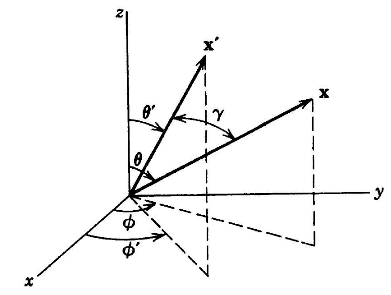
\includegraphics[scale=0.7]{Imagenes/Teorema_Adicion_01.png}
    \caption{Los dos vectores $\va{r}$ y $\va{r}^{\, \prime}$ se indican en la figura por $x$ y $\pderivada{x}$, respectivamente. El ángulo entre los dos vectores se indica por $\gamma$.}
    \label{fig:figura_01}
\end{figure}
El ángulo entre estos dos vectores, identificado por $\gamma$, se calcula fácilmente. Observando que los vectores unitarios están dados por:
\begin{align*}
\vu{r} = \sin \theta \, \cos \phi \, \vu{i} + \sin \theta \, \sin \phi \, \vu{j} + \cos \theta \, \vu{k}
\end{align*}
y de manera similar para el vector $\vu{r}^{\, \prime}$, se sigue entonces que:
\begin{align}
\cos \gamma = \va{r} \cdot \va{r}^{\, \prime} = \cos \theta \, \cos \pderivada{\theta} + \sin \theta \, \sin \pderivada{\theta} \, \cos \big( \phi - \pderivada{\phi} \big)
\label{eq:ecuacion_021}
\end{align}

El \emph{teorema de la adición para los armónicos esféricos} es:
\begin{align*}
\setlength{\fboxsep}{3\fboxsep}\boxed{
P_{\ell} (\cos \gamma) = \dfrac{4 \pi}{2 \ell + 1} \, \nsum_{m=-\ell}^{\ell} Y_{l}^{m} (\theta, \phi)^{*} \, Y_{l}^{m} (\theta, \phi) }
\end{align*}
\end{document}